\chapter{Deeplearning4j (unfinished)}
{See also \cite{DL4J}\\
von http://deeplearning4j.org/quickstart\\
DL4J targets professional Java developers who are familiar with production deployments, IDEs and automated build tools.\\

How to:
http://deeplearning4j.org/documentation
...

\section{Getting started (unfinished)}
von http://deeplearning4j.org/quickstart\\

\subsection{Vorraussetzungen und Empfehlungen (unfinished)}
- Java 1.7 oder höher (nur 64-Bit Version wird unterstützt\\
- Apache Maven (Maven is a dependency management and automated build tool for Java projects.) check https://books.sonatype.com/mvnex-book/reference/public-book.html for how to use\\
- IntelliJ IDEA oder Eclipse (An Integrated Development Environment (IDE) allows you to work with our API and configure neural networks in a few steps. We strongly recommend using IntelliJ, which communicates with Maven to handle dependencies.)\\
- Git

\subsection{Installation (unfinished)}
http://deeplearning4j.org/gettingstarted
Follow the ND4J Getting Started instructions to start a new project and include necessary POM dependencies.
http://nd4j.org/getstarted.html
http://nd4j.org/dependencies.htm

\subsection{Ein neues Projekt in IntelliJ (unfinished)}
http://nd4j.org/getstarted.html
In IntelliJ
- File -> new -> Project
\renewcommand{\figurename}{Abb.}
\begin{figure}[htp]
%%\begin{floatingfigure}[r]{textwidth}
\centering
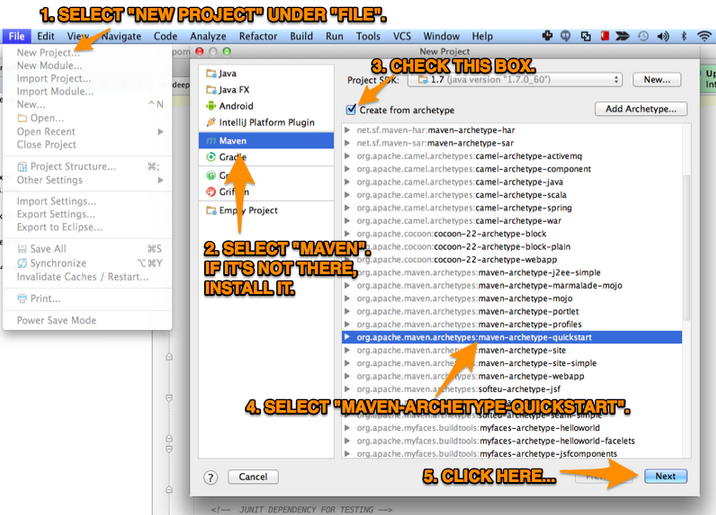
\includegraphics[width=0.60\textwidth]{pictures/new_maven_project.png}
\caption[Neues Maven Projekt]{Neues Maven Projekt erstellen\protect\footnotemark}
%%\end{floatingfigure} 
\end{figure}
\footnotetext{Quelle: ND4J \url{http://nd4j.org/getstarted.html}}
- GroupId(PackageName) und ArtifactId (Projektname?) festlegen
- Finish

- gehe ins POM.xml file
Update the POM file with the dependences you’ll need. These will vary depending on whether you’re running on CPUs or GPUs.

The default backend for CPUs is nd4j-native. You can paste that into the $<$dependencies$>$ ... $<$/dependencies$>$ section of your POM like this:
\lstset{language=XML}
\begin{lstlisting}[language=XML,caption=applicationContext.xml]
 <dependency>
   <groupId>org.nd4j</groupId>
   <artifactId>nd4j-native</artifactId>
   <version>${nd4j.version}</version>
 </dependency>
\end{lstlisting}
nd4j-cuda-7.5 (for GPUs)

ND4J’s version is a variable here. It will refer to another line higher in the POM, in the $<$properties$>$ ... 
$<$/properties$>$ section, specifying the nd4j version and appearing similar to this:
\begin{lstlisting}[language=XML,caption=applicationContext.xml]
  <nd4j.version>0.4-rc3.9</nd4j.version>
  <dl4j.version>0.4-rc3.10</dl4j.version>
\end{lstlisting}

The DL4J dependencies you add to the POM will vary with the nature of your project.

In addition to the core dependency, given below, you may also want to install deeplearning4j-cli for the command-line interface, deeplearning4j-scaleout for running parallel on Hadoop or Spark, and others as needed.
\begin{lstlisting}[language=XML,caption=applicationContext.xml]
	   <dependency>
	     <groupId>org.deeplearning4j</groupId>
	     <artifactId>deeplearning4j-core</artifactId>
	     <version>${dl4j.version}</version>
	   </dependency>
\end{lstlisting}






\section{Ein Netz erstellen und trainieren (unfinished)}
http://deeplearning4j.org/quickstart.html
Everything starts with a MultiLayerConfiguration, which organizes those layers and their hyperparameters.
Hyperparameters are variables that determine how a neural network learns. They include how many times to update the weights of the model, how to initialize those weights, which activation function to attach to the nodes, which optimization algorithm to use, and how fast the model should learn. This is what one configuration would look like:
\begin{lstlisting}
    MultiLayerConfiguration conf = new NeuralNetConfiguration.Builder()
        .iterations(1)
        .weightInit(WeightInit.XAVIER)
        .activation("relu")
        .optimizationAlgo(OptimizationAlgorithm.STOCHASTIC_GRADIENT_DESCENT)
        .learningRate(0.05)
        // ... other hyperparameters
        .backprop(true)
        .build();
\end{lstlisting}
With Deeplearning4j, you add a layer by calling layer on the NeuralNetConfiguration.Builder(), specifying its place in the order of layers (the zero-indexed layer below is the input layer), the number of input and output nodes, nIn and nOut, as well as the type: DenseLayer.
\begin{lstlisting}
        .layer(0, new DenseLayer.Builder().nIn(784).nOut(250)
                .build())
\end{lstlisting}
Once you’ve configured your net, you train the model with model.fit.

Configuring the POM.xml File

To run DL4J in your own projects, we highly recommend using Maven for Java users, or a tool such as SBT for Scala. The basic set of dependencies and their versions are shown below. This includes:

   -  deeplearning4j-core, which contains the neural network implementations
   -  nd4j-native, the CPU version of the ND4J library that powers DL4J
    - canova-api - Canova is our library vectorizing and loading data



http://deeplearning4j.org/gettingstarted.html
Reproducible Results

Neural net weights are initialized randomly, which means the model begins learning from a different position in the weight space each time, which may lead it to different local optima. Users seeking reproducible results will need to use the same random weights, which they must initialize before the model is created. They can reinitialize with the same random weight with this line:

\begin{lstlisting}
   Nd4j.getRandom().setSeed(123);
\end{lstlisting}

\subsection{RNN code (unfinished)}

\subsection{LSTM code (unfinished)}
A commented example of a Graves LSTM learning how to replicate Shakespearian drama, and implemented with Deeplearning4j
\subsubsection{Hyperparameter Tuning}
http://deeplearning4j.org/lstm.html
Here are a few ideas to keep in mind when manually optimizing hyperparameters for RNNs:
   - Watch out for overfitting, which happens when a neural network essentially "memorizes" the training data. Overfitting means you get great performance on training data, but the network’s model is useless for out-of-sample prediction.
   - Regularization helps: regularization methods include l1, l2, and dropout among others.
    -So have a separate test set on which the network doesn’t train.
   - The larger the network, the more powerful, but it’s also easier to overfit. Don’t want to try to learn a million parameters from 10,000 examples – parameters > examples = trouble.
  -  More data is almost always better, because it helps fight overfitting.
  -  Train over multiple epochs (complete passes through the dataset).
   - Evaluate test set performance at each epoch to know when to stop (early stopping).
  -  The learning rate is the single most important hyperparameter. Tune this using deeplearning4j-ui; see [this graph] %%(http://cs231n.github.io/neural-networks-3/#baby)
  -  In general, stacking layers can help.
  -  For LSTMs, use the softsign (not softmax) activation function over tanh (it’s faster and less prone to saturation (~0 gradients)).
  -  Updaters: RMSProp, AdaGrad or momentum (Nesterovs) are usually good choices. AdaGrad also decays the learning rate, which can help sometimes.
   - Finally, remember data normalization, MSE loss function + identity activation function for regression, Xavier weight initialization


} %% Ende Chapter{Deeplearning4j}